\section{Směrování}\label{prijmiEthernetove}
Směrování implementoval kolega, nicméně se Cisco nechová vždy stejně, a tak bylo nutné vyčlenit rozhodování o příjmu paketů do koncových počítačů a implementovat je každý zvlášť. Nejsložitější bylo zjistit, jak se Cisco přesně chová a proč to tak je.

Vezměme si následující síť \ref{fig:sit_2pc} složenou pouze ze dvou počítačů.

\begin{figure}[h]
\begin{center}
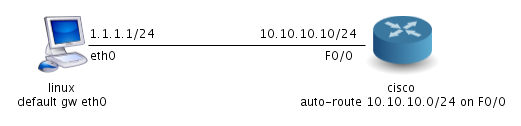
\includegraphics[width=12cm]{figures/sit_2pc.png}
\caption{Síť linux - cisco}
\label{fig:sit_2pc}
\end{center}
\end{figure}




\section{Wrapper směrovací tabulky}

\section{Překlad adres}

